La asignación de números de presos a los cajones por parte del director de la prisión se puede describir matemáticamente como una permutación de los números del 1 al 100. Tal permutación es una correlación uno a uno del conjunto de números naturales del 1 al 100 consigo mismo. Una secuencia de números que después de la aplicación repetida de la permutación regresa al primer número se llama ciclo de la permutación. Toda permutación se puede descomponer en ciclos disjuntos , es decir, ciclos que no tienen elementos comunes. 
\begin{figure}[H]
\begin{subfigure}{0.49\textwidth}
     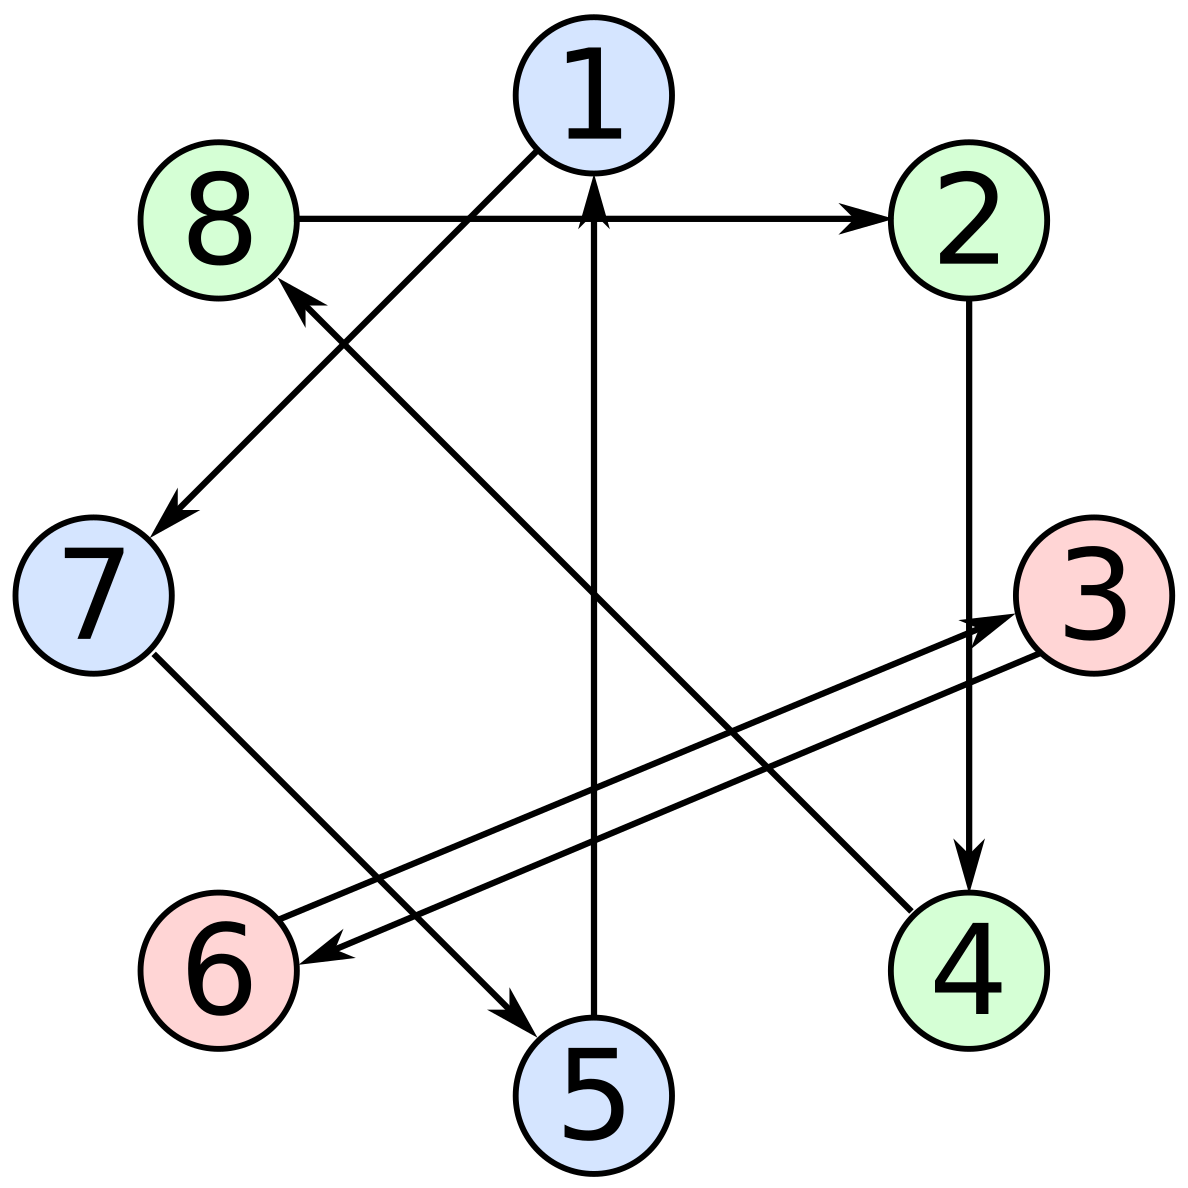
\includegraphics[width=\textwidth]{imagenes/Permutation_cycles_qtl1.png}
     \caption{Grafo del ejemplo 1}
     \label{fig:grafo_primer_ejemplo}
 \end{subfigure}
 \hfill
 \begin{subfigure}{0.49\textwidth}
     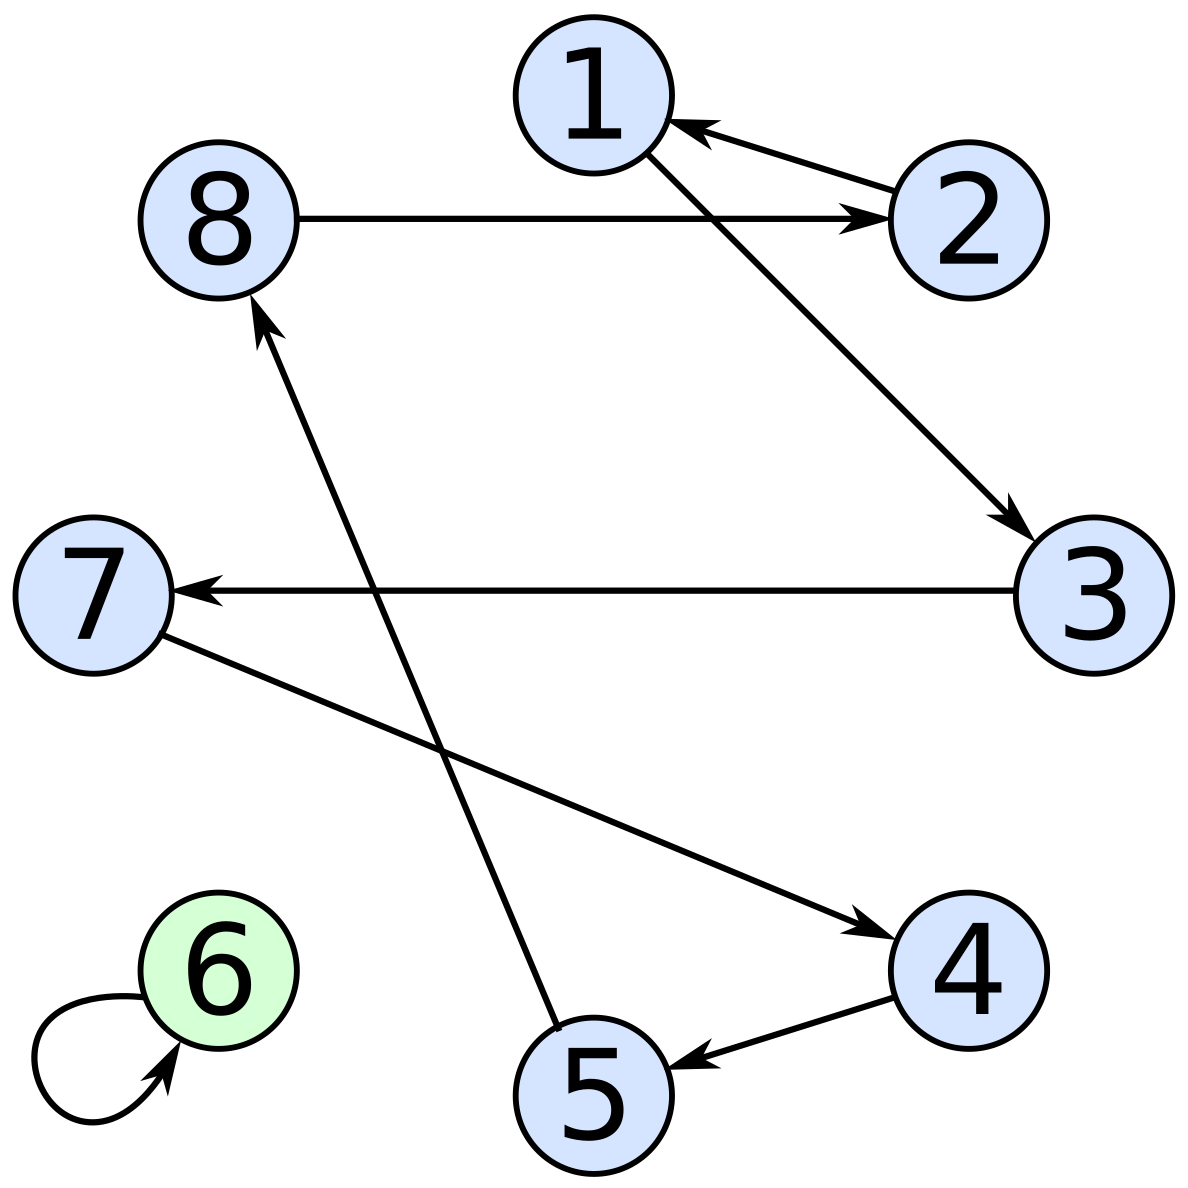
\includegraphics[width=\textwidth]{imagenes/Permutation_cycles_qtl2.png}
     \caption{Grafo del ejemplo 3}
     \label{fig:grafo_tercer_ejemplo}
 \end{subfigure}

 \caption{Representación de las permutaciones con grafos}
 \label{fig:grafos}

\end{figure}

La permutación del primer ejemplo anterior(\ref{fig:grafo_primer_ejemplo}) se puede escribir en notación cíclica como $(1 7 5)(2 4 8)(3 6)$ y por lo tanto consta de dos ciclos de longitud 3 y un ciclo de longitud 2. La permutación del tercer ejemplo(\ref{fig:grafo_tercer_ejemplo}) es en consecuencia
$(1 3 7 4 5 8 2)(6)$ y consta de un ciclo de longitud 7 y un ciclo de longitud 1. La notación del ciclo no es única ya que un ciclo de longitud l se puede escribir en l diferentes formas dependiendo del número de inicio del ciclo. Durante la apertura de los cajones en la estrategia anterior, cada preso sigue un solo ciclo que siempre termina con su propio número. En el caso de ocho reclusos, esta estrategia de seguimiento de ciclos tiene éxito si y solo si la duración del ciclo más largo de la permutación es como máximo 4. Si una permutación contiene un ciclo de 5 o más longitudes, todos los reclusos cuyos números se encuentran en dicho ciclo no alcanza su propio número después de cuatro pasos.